\documentclass[a4, conference]{IEEEtran}
\renewcommand\IEEEkeywordsname{Keywords}
\usepackage{graphicx}%balicky nevyhnutne k vytvoreniu PDF suboru
\usepackage{cite}
\usepackage{url}
\usepackage{graphicx}
\usepackage[T1]{fontenc}
\usepackage{array}
\usepackage{dblfloatfix}
\usepackage{float}

\newcolumntype{M}[1]{>{\centering\arraybackslash}m{#1}}
\newcolumntype{N}{@{}m{0pt}@{}}

% correct bad hyphenation here
\hyphenation{}

\begin{document}%zaciatok dokumentu

\title{Domain Model Relations Discovering in Educational Texts based on User Created Annotations}%nadpis clanku

\author{%hlavicka dokumentu, autor, skola,email ...
\IEEEauthorblockN{Vladim\'{i}r Mih\'{a}l, M\'{a}ria Bielikov\'{a} }
\IEEEauthorblockA{  Faculty of Informatics and Information Technologies\\
			 Slovak University of Technology in Bratislava\\
 			 Ilkovicova 3, 842 16 Bratislava, Slovakia,\\
			xmihalv@stuba.sk, bielik@fiit.stuba.sk}
}
% make the title area
\maketitle

\begin{abstract}%abstrakt dokumentu
\textbf{ Domain model with its metadata is essential part of every adaptive educational system. At the same time it is often a bottleneck as quality metadata is essential requirement and their manual creation is difficult or even impossible in some extent. So any effort in automated acquisition of metadata is crucial for effective learning supported by an educational system. In this paper we propose a method of discovering relations in educa- tional texts using annotations created by users (learners). As annotations we use links to external educational resources related to educational texts. We integrate external resources into the learning course and analyze their content. Based on the content analysis we construct a graph consisting of educational content, external resources and existing concepts in the domain model and use graph algorithms to derive new relations. Besides the benefit of discovered relations, our approach enriches educational content with additional information resources.}
\end{abstract}
\begin{IEEEkeywords}%klucove slova
adaptive educational web-based system, domain model, concepts relationships, external resources, personalization, metadata discovery, annotations
\end{IEEEkeywords}
\IEEEpeerreviewmaketitle
\section{Introduction}%zaciatok sekcie 1.
With emergence of the Web 2.0 paradigm web applications started to focus on a user and emphasized user created content. Current web-based educational systems follow this trend and strive to provide personalized content for students and support students and teachers with the means to collaborate and contribute to the content. Consequently the role of the student within educational environment evolved from a passive perceiver of information to active participant and contributor to the educational content.

To employ personalization it is necessary to create and maintain a domain model and to connect the domain model to the educational content presented to a learner. Personalized recommendation of educational content also depends on the domain model representing the content metadata. However, manual creation of quality domain model requires an expert knowledge of the domain and substantial amount of time and effort. In fact, this represents a bottleneck of most adaptive web-based educational systems. Therefore it is necessary to support creation of the domain model and automate at least some parts of the process of domain model creation.

One of approaches to the content together with a source of metadata creation is annotations created by users \cite{ref:barlatowards,ref:moro2011towards }.%pomocou prikazu \cite{} odkazujeme na referenciu uvedenu na konci dokumentu
Users create annotations within the selected regions of text and insert typically textual data (e.g. comments) often mixed together with marking parts of the content. Annotations can enrich the document with various types of metadata, such as comments \cite{ref:bielikova2010alef }, tags \cite{ref:bao2007optimizing }, or other textual supplements such as questions \cite{ref:unvcik2010annotating }. Special case of annotation is marking an important region within the educational content \cite{ref:kim2008spatial }, which can serve for example for later review of the content. Educational systems employ user created annotations to support active participation of students within a learning process \cite{ref:vsimko2011supporting } and leaving a feedback to teachers.

While annotations represent metadata attached to the content, they can also reflect importance of a portion of the content linked with inserted annotations. Moreover, the same or similar annotations are frequently inserted into various regions of educational content (e.g., same or similar tags inserted into several different parts of the document). By inserting annotations in such manner, users express that annotated parts of the document describe possibly similar topics. Consequently user created annotations can be used to discover relations between various parts of educational content.

In this paper we present a method for enriching educational content together with its domain model by inserting links into related external information resources. Students or teachers can insert links into the educational content. We integrate the links into educational course (within particular learning objects), extract metadata from the content of linked external documents and use the extracted metadata to discover relations between learning objects in the domain model.

We evaluated our method within ALEF-a web-based adaptive learning framework designed to support collaboration, content creation and personalization. We implemented our method for enriching educational content by external resources and used in autumn semester 2010/11 in the Procedural Programming course. As a result we evaluated the method using real world data.

The paper is structured as follows. First, we discuss related work of metadata creation for the web content. Next, in Section 3 we describe the ALEF framework as a basis for realization of proposed method. Section 4 presents our method for discovering relations based on external resources. We evaluate our method in Section 5 and conclude with our Conclusions. 
\section{RELATED WORK}%zaciatok sekcie 2.
%
There are several approaches to creation of metadata on the Web. Some approaches rely on automated processing of the texts, detecting keywords, named entities or concepts and using various text mining metrics to discover relation between identified keywords \cite{ref:vsimko2011supporting }. Others use metadata created by users (e.g. tags), to characterize resources and users \cite{ref:hunter2008harvana } and use acquired metadata to improve search \cite{ref:bao2007optimizing }, personalize navigation \cite{ref:farzan2008annotated }or adaptively recommend content \cite{ref:shepitsen2008personalized } to users.

Automated generation of the domain model from the educational texts relies on identifying keywords in the text. In \cite{ref:vsimko2011supporting } authors extract and analyze keywords to find relatedness of particular keyword to the whole domain which is described by the corpus of educational texts. Keywords with relatedness value higher than the threshold are chosen as pseudo-concepts. Afterwards, similarity between concepts using various graph algorithms is counted.

Another approach uses latent semantic analysis to discover relationships between web pages \cite{ref:macedo2002infrastructure }. After discovering relations between documents, they created hyperlinks between documents and inserted them into documents. Authors presented their research as a part of infrastructure for organizing web documents, managing links and providing link- related services. Thus they provide a separate layer of links, which are stored in the separated link bases eliminating the need of changing content of underlying documents

Metadata manually created by users are typically represented as user created annotations. A user created annotation can be defined as a triplet (u, r, m), where u is a user, r a resource, which is being annotated and m represents metadata inserted by the annotation \cite{ref:shepitsen2008personalized }. It is possible to use a vector of annotations inserted by certain user to express interests of that user. Similar vector can be used to describe resources and using a similarity measure to evaluate most relevant resources to the user, or rank concepts present in the domain model \cite{ref:vsaloun2010evaluation }.

When used in learning, annotations created by users increase motivation of students to use educational system and to more actively participate within the learning process \cite{ref:bielikova2010alef }. One of the important conclusions of research regarding annotations is that it is essential to motivate students to insert quality annotations. One way to motivate students is through the value of annotations. If annotations provide benefits to students almost instantly after inserting (e.g., creating useful side-notes, highlighting important portions of a text) students will insert annotations to take advantage of them. Naturally, one should consider also rewarding students for creating quality annotations \cite{ref:moro2011towards }.

Another significant aspect of annotations is their speciali- zation. Simple text comment annotations can be used in various ways what can lead to inconsistent metadata, while more special annotations with clear purpose (e.g., tags, important regions of text) provide less ambiguous metadata. It is also important to consider and clearly explain users the purpose of the annotations, so they insert correct annotations.

While annotations in educational systems are widely used as a mean to support communication and collaboration, the 
potential to create a metadata and contribute to the educational content is typically unexploited. We believe that annotations inserted into educational content represent valuable source of educational metadata which can help various methods of adaptive learning to function more efficiently.
\section{ALEF - ADAPTIVE LEARNING FRAMEWORK }%zaciatok sekcie 3.
% 
ALEF is a web-based adaptive learning framework designed especially to support collaborative learning and problem solving, content creation by students and personalization of educational content. It also provides personalized recommendation, embedded interactive content such as test questions included in learning objects and supports automated domain and knowledge modeling. ALEF is currently used for learning programming (C, lisp and prolog languages) and principles of software engineering in several bachelor learning courses.

Collaboration features of ALEF allow adding various types of content annotations: comments, tags, bug reports, questions and external resources. Students are motivated to actively participate in the content enrichment by these annotations through gaining score points, which creates a competition through presenting score and rank for each student (see Fig.\ref{obrazok1}).%pomocou prikazu \ref{obrazok1} odkazujeme na obrazok1

To further encourage students to insert annotations, ALEF provides possibility to change the level of the annotation visibility. Students choose among following levels of visibility:
\begin{itemize}%vytvorenie zoznamu s odrazkami
\item public 
\item public anonymous 
\item private 
\end{itemize}
Public annotations are visible to all students. Public anonymous annotations are also visible to all students but name of user who inserted the annotation is replaced with ``Anonymous''. Private annotations are visible only to users who inserted them. In this paper we concentrate on specific kind of annotations, which allow for extending educational content - external resources.  
\section{METHOD FOR DISCOVERING RELATIONS BASED ON EXTERNAL RESOURCES}%zaciatok sekcie 4.
%  
In addition to using regular educational resources provided by a teacher, students typically search the Web for additional information resources. Information resources on the Web are attractive to students, since they often offer alternative view and thus better understanding difficult parts of the content or contain example solutions to problems given for homework. Students obviously share the most useful resources among each other through various discussion forums. However, searching and sharing resources is separated from the learning process and it depends entirely on communication between students.

We provide students with a possibility to link interesting information resources into the educational content (actual learning objects) and share them with their peers within the educational course. In such a way we improve availability of information resources to all students, encourage students to search the Web for additional information resources and thus improve overall learning experience. Annotations represent a convenient way to insert links to external information resources, which serve also as a source of metadata for related educational content.

It is necessary to clearly define the purpose and properties of annotations. In case of inserting links to external resources it is crucial to emphasize the relatedness of external resource
\begin{figure*}%vlozenie obrazku do dokumentu
\centering
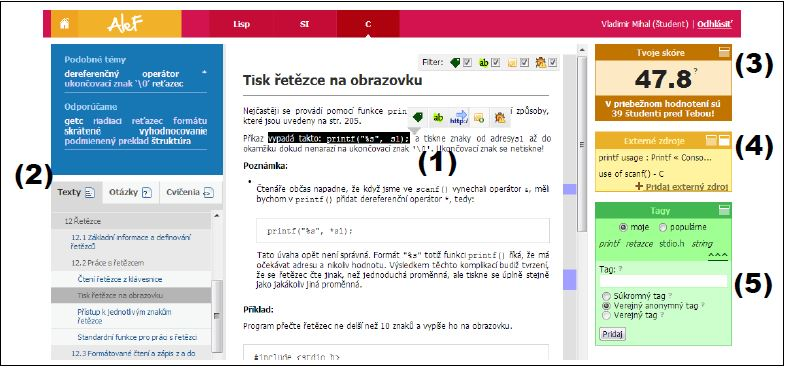
\includegraphics [width=\textwidth]{Figure1.jpg}
\caption{Example screenshot of ALEF (interface in Slovak, educational texts in Czech). Educational content, which is enriched with interactive content and annotations is presented in the middle part of the screen (1), navigation, either through menu or through recommendations, is on the left part (2) and collaboration tools such as score achieved by student (3) external sources (4) and tags (5) inserted into current learning object.}
\label{obrazok1}
\end{figure*}
to the whole educational course and to the document (learning object) where the link is inserted. After inserting a link into the related educational content, the link becomes integrated into the content thus easier accessible to students.

External resources inserted into the educational content describe similar concepts as the text of particular learning object does. Hence we can process the resources, detect which concepts they describe and assume that these concepts are related to the learning object they extend. We can also assume that concepts which co-occur in numerous external resources are closely related.

We proposed a method to extract metadata from external resources inserted into the educational text and use the acquired metadata to enrich existing domain model. It consists of the following steps:
\begin{enumerate}%vytvorenie zoznamu s cislami
\item Annotating educational content by external resources  
\item Processing the content of external resources 
\item Enhancing domain model by discovering relations
\end{enumerate} 
In the first step users insert related links to learning objects. Links can be inserted either by a teacher (e.g., for motivating students to study beyond the learning course) or students (to share interesting information sources with peers). Users also rate inserted sources expressing their usefulness and relatedness to the educational content. Ratings provide us \textbf {indirect information about potential quality of resources.} We calculate ratings for inserted external resources by students separately from ratings submitted by teachers; teacher\textsc{\char39}s ratings have higher trust than rating from students.

Goal of the second stage is to process the content of external resources, detect concepts which are explained or mentioned in the content and create weighted relations between external resources and detected concepts.  Goal of the second stage is to process the content of external resources, detect concepts which are explained or mentioned in the content and create weighted relations between external resources and detected concepts.

Since the links are inserted entirely by users, we do not have any prior knowledge about the content or format of external resource. Useful external resource can be practically in any language or format (e.g., text, picture, video, presentation) as long as it helps students to understand related learning topic. To overcome this issue we perform a preprocessing, \textbf {which consists of extraction of readable text from the source} depending on type of the source and translating textual content to English as for English several efficient methods for text processing exist (together with corresponding software tools realizing the methods). To improve efficiency of further processing of external resources we represent their content as weighted set of words.

After the content analysis we construct a graph where learning objects, concepts and external resources are nodes and relations represent edges. Edges of the graph are constructed from known relations - external resources inserted into learning objects and concepts identified in external resources.As a result we get a tripartite graph with learning objects and concepts on the sides connected through external resources.

In the third step we use graph algorithms to find similarity between learning objects and concepts and discover new In the third step we use graph algorithms to find similarity between learning objects and concepts and discover new relations for the domain model. We use spreading activation algorithm to calculate a distance of concepts and learning objects from particular learning objects. We spread the activation from the learning object nodes to the concepts through external resource nodes. 
\subsection{Processing the Content of External Resources }%zaciatok 1. podsekcie
% 
To identify concepts within an external resource we use string matching algorithm. We search the content of external resource for occurrences of concepts from existing domain model and for every concept, which is found in the resource we create a weighted relation. We match each word from the content of external resource against concepts and count similarity between them. If similarity of the word with a concept is higher than matching threshold we state the word as an occurrence of the concept.

We define the similarity function of two words $w_{1}$ and $w_{2}$:
\begin{equation}%vytvorenie vyrazu, rovnice, nejakeho vztahu
sim(w_{1},w_{2})= 1-\frac{ldist(w_{1},w_{2})}{max lenght(w_{1},w_{2})}
\end{equation}

where ldist($w_{1}$, $w_{2}$) denotes function for weighted Levenshtein (edit) distance of given words. If a concept contains more than one word we match each word separately.

After matching separate concept words we average number of matches using harmonic mean, since such averaging penalizes frequently occurring concept words (which are typically general) in favor of more specific and therefore more valuable. We also further penalize those multi word concepts containing words which are never matched in the external resource, because those concepts are probably unrelated to the resource, so all identified matches of the concept are aforementioned nonspecific concept words.

To calculate the weight of identified concepts we defined the weight function: 
\begin{equation}
w(c,ext) = \frac{occ(c,ext)}{\arrowvert id(ext)\arrowvert ln(lenght(ext))}
\end{equation}

where \textit{occ(c, ext)} denotes number of identified occurrences of the concept c in the external resource ext.  id(ext) represents a set of all identified concepts within the external resource ext. We normalize the weight of concept by natural logarithm of document length to resolve issues with long external resources, which usually cover great number of concepts.

As last step of the content analysis we reduce the set of identified concepts to contain only most significant ones. We defined a function (3) to calculate n, the number of concepts with highest weight which should be assigned to external resource ext, while length (ext) represents a length of external resources content in number of words and k is a parameter to adjusting the rate of reduction of assigned concepts.

\begin{equation}
n=\sqrt{\frac{length(ext)}{k}}
\end{equation}

Result of the content processing step is that every external resource has assigned a weighted set of concepts which are contained within a content of the source. This set represents relations between external resource and concepts. 
\subsection{Deriving new relations}%zaciatok 2. podsekcie
% 
After successful analysis of external resources\textsc{\char39} content we construct a tripartite graph in which learning objects, concepts and external resources are nodes while already known relations are edges. Fig.\ref{obrazok2} shows an example of such graph.

To derive new relations we apply spreading activation on the constructed graph. We calculate similarity of concepts and learning objects to each other. To create relations based on the similarity we select nodes with highest energies. We use also normalized values of energies to calculate weights of created relations.

We calculate following types of weighted similarities:
\begin{enumerate}
\item \textit{Learning object - Learning object} 
\item \textit{Concept - Concept} 
\end{enumerate}
We identified the type of discovered relations between two
\begin{figure}[H]
\centering
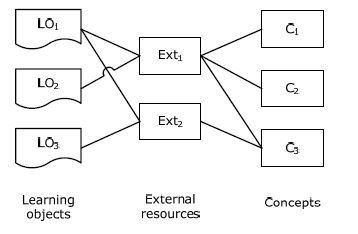
\includegraphics [width=\linewidth]{Figure2.jpg}
\caption{Graph of learning objects, concepts and external resources constructed from known relations.}
\label{obrazok2}
\end{figure}
concepts as related-to relation, since various concepts co-occur in many external resources and they are related. However we cannot specify relation between two concepts more precisely. Type of discovered relations between two learning objects we identified as similar-to. Learning objects with several common external resources are probably explaining very similar concepts (e.g. while and for loops for procedural programming domain). Such learning objects can be useful when studied in one learning session (texts first, then questions and exercises). 
\section{EVALUATION}
%  
To collect external resources we implemented functionality of collecting and processing external resources and deployed it within ALEF. We created a sidebar widget for inserting and browsing external resources (see Fig. \ref{obrazok3}). Students can easily insert a new external resource into currently presented learning object by providing an URL of the source and an optional comment. We also keep possibility to insert external resources through a text selection context tooltip, since it is a default way to insert annotations in ALEF.

The sidebar widget displays links to external resources attached to current learning object. They are sorted by their 
\begin{figure*}
\centering
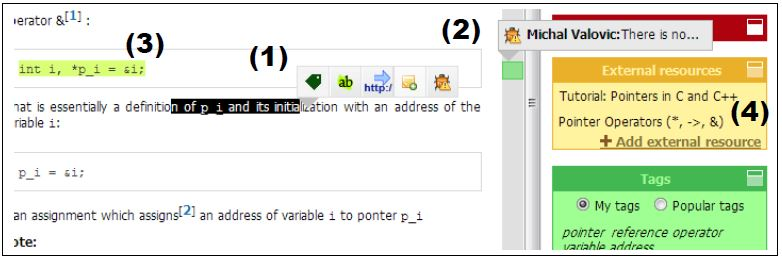
\includegraphics [width=\textwidth]{Figure3.jpg}
\caption{Annotations within ALEF framework. Tool tip for inserting various types of annotations: (from leftmost) tags, highlights of important parts of the text, external sources, text comments and reports of an errors (1), annotation reporting error in the educational content (2), highlighted important portion of educational text (3) and widget for inserting and displaying external sources (4).}
\label{obrazok3}
\end{figure*}
ratings gained from students and teachers. To reduce possible information overhaul we reduce their count in the default view only to three highest rated sources.

To increase students\textsc{\char39} motivation we employed a student score assessment, which was already implemented within ALEF. We reward students with score points for every inserted link and every rating of external resources usefulness. We additionally reward students whose external resources were quality and useful ones (according to ratings) and penalized those who inserted links unrelated websites.

Students used the ALEF framework during the Procedural programming course in autumn semester 2010/11 providing us a possibility to collect annotations and feedback from real users in real world deployment environment. We deployed functionality of external resources within the course from December 1st, 2010 to January 15th, 2011. We initially inserted 57 external resources to demonstrate the newly deployed functionality and to motivate students to insert sources they discovered. During the deployment period we collected 742 external resources from 42 students.

While collecting rather large number of external resources, students left us only 610 useful ratings for all resources, what makes only 0.82 ratings per source. Since it is clearly not sufficient number of ratings for further evaluation of the method, we discarded these ratings.

Because of the lack of ratings of quality and a large amount and varying quality of collected external resources as well, we created a subset of collected external resources solely for purposes of evaluation. We manually selected 117 selected external resources into the experimental set. To each of selected sources we manually assigned usefulness rating.

We automatically processed content of each source from the set and assigned related concepts from the domain model, which were consequently evaluated by a domain expert (teacher). We choose to identify concepts from the domain model automatically created for the Procedural programming course. We also analyzed and compared discovered relations against the generated model. Task of the expert was to select which concepts are identified correctly and which wrongly. We calculated precision of the concept identification as a ratio of correct concepts to all concepts. Concept identification gained 74.8 percent precision, which we found sufficient.

\begin{table}[ht]%vytvorenie tabulky
%\setlength\extrarowheight{7pt}
\renewcommand{\arraystretch}{2.5}
\small
\centering
\caption{RESULTS OF EVALUATION OF DISCOVERED RELATIONS.}
\label{tabulka1}
%\label{my-label}
\begin{tabular}{|M{3cm}|M{3cm}|N}
\hline
\textbf{Type of relation} & \textbf{precision}
\\ \hline 
Learning objects          & 81.34\%      
\\ \hline
Concepts                  & 72.47\%        
\\ \hline
\end{tabular}
\end{table}
Relations between concepts and between learning objects based on similarities we evaluated in similar manner. Precision of discovering new relations is presented in Tab.\ref{tabulka1}.

After analysis of correctly identified relations between pairs of learning objects we discovered that significant portion of discovered relations was already presented in the domain model - they represent relations between parts of document in the hierarchy (e.g., relations between a chapter and its sections). Relations which were not already included within the domain model connected educational texts with related interactive questions or exercises. While such relations seem to be beneficial, for instance for the content recommendation, these relations can be derived from the domain model itself without need of any annotations. Because for every learning object exist defined relations with concepts which it explains, it is possible to connect related learning objects through the concepts what results into the relations similar to ours.

While precision of relation identification between pairs of concepts was lower, we discovered more correct relations not previously contained in the domain model. In case of relations between concepts, it is not as straightforward to derive such relations from existing domain model. Hence we believe that relations between concepts discovered by our method represent possible enrichment to domain model of educational web- based system and present viable extension to the method of automatic domain model generation already realized in the ALEF framework \cite{ref:vsimko2009automated }. 
\section{CONCLUSIONS}
%  
We proposed a method for discovering relations between concepts in a domain model of web-based adaptive educational system based on an enrichment of educational content by external resources. It is a part of collaborative flow in the adaptive learning framework ALEF developed at the Slovak University of Technology in Bratislava. Evaluation of our method showed that it derives correct relations between concepts and learning objects, which can be used as metadata in personalization of educational materials. However, quality of derived relations highly depends on the processing of external resources.

Precision of relation identification can be further improved with manual aid of an expert. Since the effort required for concept evaluation was minimal in contrast to manual creation of relations, we assume that designed method can be used as a semi-automatic way to enrich a domain model or as an aid to manual creation or modification of domain model.

Besides the benefit of discovered relations between concepts in the domain model, external resources interlinked within learning objects  
\begin{itemize}
\item enrich the content of an educational course
\item provide students with additional information resources to study 
\item motivate for active learning
\end{itemize} 
For the most motivated and skilled students it presents an opportunity to expand their knowledge. Linked resources can be also processed by more advanced methods of content analysis and processing (e.g., summarization or identification of interesting fragments) and possibly presented interactively within educational texts in an educational system, in same way as questions and exercises are currently presented in our ALEF framework.
\section*{ACKNOWLEDGMENTS}%zaciatok 6.sekcie, 
%  
This work was partially supported by the grants VG1/0675/11/2011-2014, KEGA 028-025STU-4/2010 and it is the partial result of the Research and Development Operational Programme for the project Research of methods for acqui- sition, analysis and personalized conveying of information and knowledge, ITMS 26240220039, co-funded by the ERDF.

The authors wish to thank all members of the ALEF development team (members of Personalized Web group, pewe.fiit.stuba.sk) for their invaluable contribution to the ALEF framework realization and deployment and helping with experiments during its use in several courses at the Slovak University if Technology in Bratislava, Faculty of Informatics and Information Technologies. 
\bibliographystyle{IEEEtran}
\bibliography{ref}
\end{document}
